\chapter{Persisting Highscores}
The game we have built so far is clearly fun to play, however, if we want
players to come back regularly we will need a highscore feature. Highscores will
motivate players to improve their skills by playing the game frequently.

For this game we will keep the mechanism very simple. For each game mode we will
store the highest score the player has achieved. These scores will only be
stored locally on the device. Then we'll extend the game over popup to show the
current highscore and to inform the player in case she has beaten her old one.

\begin{details}[Why not Apple's Game Center?]
For this chapter I have considered using Apple's \textit{Game Center} framework,
which provides features such as leaderboards and achievements. I've decided
against it because it would require all readers to purchase an Apple Developer
account (required settings for Game Center games are only available fo
registered Apple Developers). If you are interested in adding \textit{Game
Center} support to your game you should read this tutorial:
\url{http://rebeloper.com/add-game-center-spritebuilder-app-swift/}
\end{details}

Before adding this feature we should, once again, talk about the architecture of
our game. Which class should be responsible for storing highscores?

Since each game mode defines its own game rules and keeps track of highscores
during the game, it should also be responsible for persisting the highscores.
 
\section{Extending the GameMode Protocol}
We'll start implementing this feature by extending the definition of the
\inlinecode{GameMode} protocol. We'll add a required method called
\inlinecode{saveHighscore}. That method will be called from within
\inlinecode{MainScene} as soon a game ends. All game modes will implement this
method and perform the highscore storing code within it.

\begin{leftbar}
Open \filemention{GameMode.swift} and add the following method to the
end of the protocol definition:
\begin{lstlisting}
func saveHighscore()
\end{lstlisting}
\end{leftbar}

Now that we've extended the definition of the protocol we need call this method
from within \inlinecode{MainScene}. Whenever a game ends, we want to store the
latest highscore of the current game mode. It makes the most sense to place this
method call in the \inlinecode{gameOver} method.

\begin{leftbar}
Extend the \inlinecode{gameOver} method in \filemention{MainScene.swift} to look
as following:
\begin{lstlisting}
func gameOver() {
  isGameOver = true
  userInteractionEnabled = false
  isDraggingPot = false
  (*@\colorbox{light-gray}{gameMode?.saveHighscore()}@*)
  presentGameOverPopup()
}
\end{lstlisting}
\end{leftbar}

This change was simple. Now let's implement the highscore saving mechanism for
both game modes.

\section{Storing Highscores for the Endless Game Mode}
iOS provides us with a variety of options to persist application data.
\textit{Core Data} offers a feature-rich object persistence API that allows for
advanced features such as search and migration between different versions of a data model. Through
\inlinecode{NSKeyedArchiver} we are able to serialize objects and store them
in files. Another option, preferred for simple tasks, is using the
\inlinecode{NSUserDefaults} class to persist information.

\inlinecode{NSUserDefaults} is a persistent key-value store with a very simple
API. Here's an example of we can store a highscore value:
\begin{lstlisting}
NSUserDefaults.standardUserDefaults().setInteger(20, forKey: "highscore")
\end{lstlisting}
All we need to provide as a key and a value - just as when working with a
dictionary. 

Retrieving the information is just as straightforward:
\begin{lstlisting}
let oldHigschore =
NSUserDefaults.standardUserDefaults().integerForKey(highscoreKey)
\end{lstlisting}

Since we only want to score one integer per game mode, this simple API is ideal
for our purposes.

Let's start with the implementation for the \inlinecode{EndlessGameMode}.

\begin{leftbar}
Add the following two member definitions to \filemention{EndlessGameMode.swift}:
\begin{lstlisting}
private let highscoreKey = "EndlessGameMode.Highschore"
private var newHighscore = false
\end{lstlisting}
\end{leftbar}

We define a variable called \inlinecode{newHighscore} to keep track of whether
or not the latest achieved score was a highscore. We will check this value when
we generate the highscore message. If the latest score was a highscore, we will
extend the message to congratulate the player.

We'll also define a constant for the \textit{key} that we use to store and
retrieve the highscore from \inlinecode{NSUserDefaults.} When defining a key for
working with \inlinecode{NSUserDefaults} it's good practice to prefix it with the current class name. That avoids conflicts between
different parts of your app that might store and access information in the user
defaults.

Now we can implement the \inlinecode{saveHighscore} method. We'll check if
the latest score is higher than the current highscore. If that's the case we
will persist the latest score and set the \inlinecode{newHighscore} variable to
\inlinecode{true}. Otherwise we'll simply set \inlinecode{newHighscore} to
\inlinecode{false}.

\begin{leftbar}
Add the following method to \filemention{EndlessGameMode.swift}:
\begin{lstlisting}
func saveHighscore() {
  let oldHigschore = NSUserDefaults.standardUserDefaults().integerForKey(highscoreKey)

  if (Int(survivalTime) > oldHigschore) {
    // if this score is larger than the old highscore, store it
    NSUserDefaults.standardUserDefaults().setInteger(Int(survivalTime), forKey: highscoreKey)
    NSUserDefaults.standardUserDefaults().synchronize()
    newHighscore = true
  } else {
    newHighscore = false
  }
}
\end{lstlisting}
\end{leftbar}

Now we are conforming to the new \inlinecode{GameModeDelegate} protocol and are
successfully storing new highscores! One interesting line that we did not
discuss yet is the following:
\begin{lstlisting}
NSUserDefaults.standardUserDefaults().synchronize()
\end{lstlisting}
This line forces \inlinecode{NSUserDefaults} to write the latest changes to disk
immediately. This method is called periodically by default. If we however store
more or less sensitive information, such as the latest highscore a player just
achieved, we call the method explicitly. That way the changes are persisted
right away, eliminating the risk of losing data if the app crashes or is quit by
the user.

Now there's a last step left. We should change the highscore message that we are
displaying at the end of the game to include the player's highscore. Further, if
the player just beat her own highscore we want to display a special message to
congratulate the player.

\begin{leftbar}
Replace the existing \inlinecode{highscoreMessage} method with the following
one:
\begin{lstlisting}
func highscoreMessage() -> String {
  let secondsText = "second".pluralize(survivalTime)

  if (!newHighscore) {
    let oldHighscore = NSUserDefaults.standardUserDefaults().integerForKey(highscoreKey)
    let oldHighscoreText = "second".pluralize(oldHighscore)
    
    return "You have survived \(Int(survivalTime)) \(secondsText)! Your highscore is \(Int(oldHighscore)) \(oldHighscoreText)."
  } else {
    return "You have reached a new highscore of \(Int(survivalTime)) \(secondsText)!"
  }
}
\end{lstlisting}
\end{leftbar}

One of the first things you might notice is that we've introduced a
\inlinecode{pluralize} method on \inlinecode{String}. This method is
part of the helpers (in \filemention{Helpers.swift}) that we've included right
at the beginning of this project. Since we now have multiple occasions in which
we need to use the pluralized form of a word, it makes sense to factor this
functionality out and avoid code duplication. This \inlinecode{pluralize} method is very primitive, it will
append and \textit{s} to a word in case the integer passed to the method is
unequal one. That is obviously not the correct way to pluralize all English 
words, but for our game in which we use \textit{points} and \textit{seconds} it
works just fine.

In the first line of this method we determine whether we need to use the word
\textit{second} or \textit{second\textbf{s}} using the \inlinecode{pluralize}
method.

Next, we check if the player has achieved a new highscore. If not, we display
the latest score along with the current highscore. Otherwise we let the player
know that he just reached a new highscore.

This is all it takes to build a simple highscore system!
\inlinecode{NSUserDefaults} can go a pretty far way when storing this kind of
simple information.

All that is left for this chapter is adding the same highscore functionality to
the timed game mode.

\section{Storing Highscores for the Timed Game Mode}
The implementation for the timed game mode is very similar to the one we've
implemented just now. In fact they are so similar that I briefly thought about
factoring the implementation out, so that it can be used by both game modes
without duplicating code. However, I've decided not to follow through on that
idea. I think the amount of duplicate code in this case isn't large enough to
require a more abstract but more complex solution. If you were to add a few more
game modes this might change, for now we are going to accept some code
duplication.

Since the implementation is so similar to what we've just seen, we won't discuss
it in the usual detail.

\begin{leftbar}
Add the \inlinecode{newHighscore} variable and the \inlinecode{highscoreKey}
constant to \filemention{TimedGameMode.swift}:
\begin{lstlisting}
private let highscoreKey = "TimedGameMode.Highschore"
private var newHighscore = false
\end{lstlisting}
\end{leftbar}
These two properties are basically the same as in the
\inlinecode{EndlessGameMode}. 

Next, add the highscore saving method for \inlinecode{TimedGameMode}.

\begin{leftbar}
Add the following method to \filemention{TimedGameMode.swift}:
\begin{lstlisting}
func saveHighscore() {
  let oldHigschore = NSUserDefaults.standardUserDefaults().integerForKey(highscoreKey)
  
  if (points > oldHigschore) {
    // if this score is larger than the old highscore, store it
    NSUserDefaults.standardUserDefaults().setInteger(points, forKey: highscoreKey)
    NSUserDefaults.standardUserDefaults().synchronize()
    newHighscore = true
  } else {
    newHighscore = false
  }
}
\end{lstlisting}
\end{leftbar}

And finally update the method that displays the highscore message.
\begin{leftbar}
Replace the existing \inlinecode{highscoreMessage} method within
\filemention{TimedGameMode.swift} with the following one:
\begin{lstlisting}
func highscoreMessage() -> String {
  let pointsText = "point".pluralize(points)
  
  if (!newHighscore) {
    let oldHighscore = NSUserDefaults.standardUserDefaults().integerForKey(highscoreKey)
    let oldHighscoreText = "point".pluralize(oldHighscore)
    
    return "You have scored \(points) \(pointsText)! Your highscore is \(Int(oldHighscore)) \(oldHighscoreText)."
  } else {
    
    return "You have reached a new highscore of \(points) \(pointsText)!"
  }
}
\end{lstlisting}
\end{leftbar}
Overall this implementation is almost identical to the Endless Game Mode's one.

\section{Summary}
Now we've implemented the entire highscore functionality for both game modes!
I'll admit that it is a very simple functionality, but it will definitely
increase the motivation of players to come back to our game. Here's what the
popup message should look like once you've finished a game:

\begin{figure}[H]
    \centering
    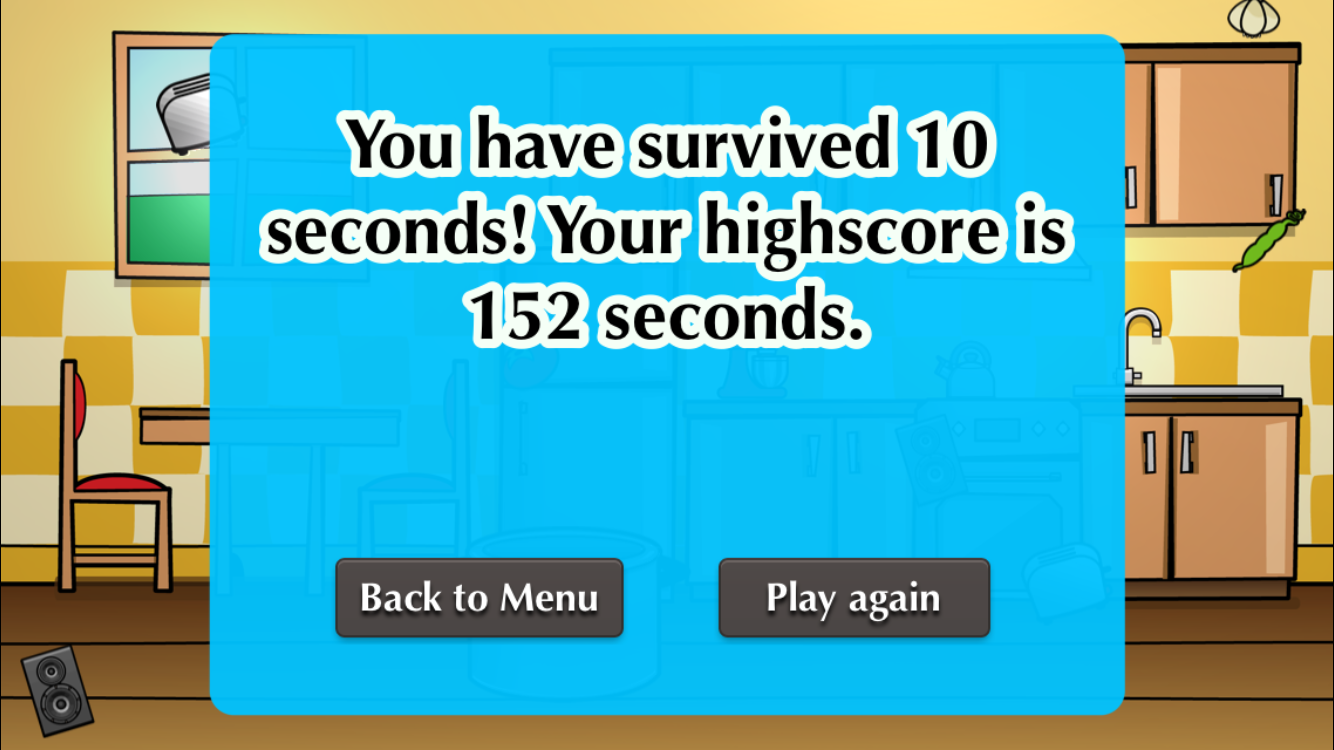
\includegraphics[width=0.6\linewidth]{images/Chapter8/Highscore_Message.png}
    \caption{When the game ends the user retrieves information about their
    highscore}
\end{figure}

We're almost done with implementing this game and thus you are getting close to
the end of this book. In the last chapter we will discuss something that makes
the difference between a good game and a fantastic one: \textit{Effects and
Animations}! Get ready for the Grand Finale.

\subsection{Grab the Source Code}
You can find the Source Code for this chapter on GitHub:
\url{https://github.com/SpriteBuilder-Book/Code/tree/master/Chapter7/}.
